\documentclass{article}
\usepackage{amsmath,amssymb}
\usepackage{graphicx}
\usepackage{enumerate}
\usepackage{hyperref}
\usepackage{subcaption}
\usepackage{caption}
\usepackage{xcolor}

\pagestyle{empty} \addtolength{\textwidth}{1.0in}
\addtolength{\textheight}{0.5in}
\addtolength{\oddsidemargin}{-0.5in}
\addtolength{\evensidemargin}{-0.5in}
\newcommand{\ruleskip}{\bigskip\hrule\bigskip}
\newcommand{\nodify}[1]{{\sc #1}}
\newcommand{\points}[1]{{\textbf{[#1 points]}}}
\newcommand{\subquestionpoints}[1]{{[#1 points]}}
\newenvironment{answer}{{\bf Answer:} \sf }{}%

\newcommand{\bitem}{\begin{list}{$\bullet$}%
{\setlength{\itemsep}{0pt}\setlength{\topsep}{0pt}%
\setlength{\rightmargin}{0pt}}}
\newcommand{\eitem}{\end{list}}

\setlength{\parindent}{0pt} \setlength{\parskip}{0.5ex}
\setlength{\unitlength}{1cm}

\newcommand{\pa}[1]{[[PA: #1]]}

\renewcommand{\Re}{{\mathbb R}}
\newcommand{\E}{{\rm E}}
\begin{document}

\pagestyle{myheadings} \markboth{}{CSCI 4302/5302 Advanced Robotics, Homework \#2, Fall 2021}

{\huge
\noindent HW \#2: Value/Policy Iteration, Discretization}\\
\ruleskip
{\bf Name}: YOUR NAME HERE\\

{\bf Deliverable}:  PDF write-up by {\bf Friday October 1st, 5:00pm}.  Your PDF should be generated by replacing the placeholder images in this LaTeX document with the appropriate solution images for each question.  Your PDF and code is to be submitted into the course Canvas. The scripts will automatically generate the appropriate images, so you only need to recompile the LaTeX document to populate it with content.

\textbf{Graduate Students:} You are expected to complete the entire assignment.\\
\textbf{Undergraduate Students:} You need only complete questions that do not have \textbf{(GRAD)} next to them. You do not need to implement max-ent Value Iteration or look-ahead policies.\\

\vspace{.1in}

You will need to install matplotlib and the OpenAI Gym Environment for Python:\\
pip install gym\\
pip install matplotlib

\vspace{.2in}

%--------------------------------------------------------------------------------
%--------------------------------------------------------------------------------
%--------------------------------------------------------------------------------
\noindent {\bf 1. Value Iteration}
%--------------------------------------------------------------------------------
%--------------------------------------------------------------------------------
%--------------------------------------------------------------------------------

\begin{enumerate}[(a)]

\item {\bf [20pts] Value iteration.} First, you will implement the value iteration algorithm for the tabular case. You will need to fill the code in \texttt{code/tabular\_solution.py} below the lines \texttt{if self.policy\_type == `deterministic\_vi'}. Run the script for the two gridworld domains and report the heatmap of the converged values.

\begin{figure}[h!]
    \centering
    \begin{subfigure}{0.45\textwidth}
        \centering
        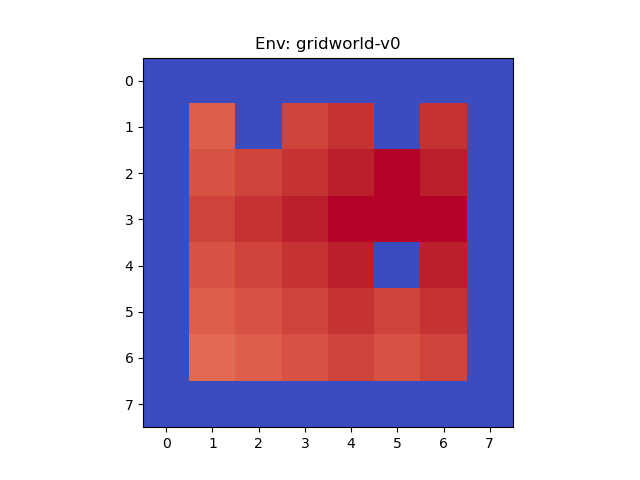
\includegraphics[width=\textwidth]{../figures/gridworld-v0_deterministic_vi.png}
        \caption{Heatmap of the final values on the \texttt{GridWorld(0)} environment.}
    \end{subfigure}
    \hspace{0.2in}
    \begin{subfigure}{0.45\textwidth}
        \centering
        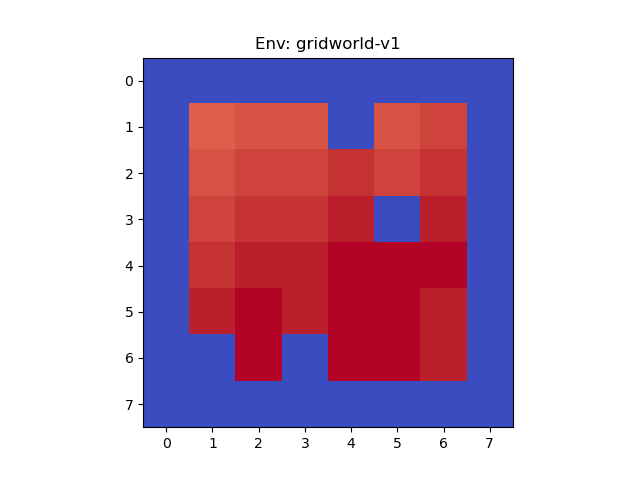
\includegraphics[width=\textwidth]{../figures/gridworld-v1_deterministic_vi.png}
        \caption{Heatmap of the final values on the \texttt{GridWorld(1)} environment.}
    \end{subfigure}
\end{figure}

\newpage 

\item {\bf [20pts] Maxent value iteration \textbf{(GRAD)}.} If our environment model isn't perfect, a deterministic policy can fail. To mitigate this problem, we introduce a stochastic policy that may try alternative actions instead of getting stuck in a given state. This distribution over actions can be obtained by using maximum entropy value iteration.  You will need to fill the code in \texttt{code/tabular\_solution.py} below the lines \texttt{if self.policy\_type == `max\_ent\_vi'}. Run the code with the maximum entropy policy and report the heatmap of the converged values for the temperature values $1, 1\text{e-}2, 1\text{e-}5$. Important implementation details, represented in the equations below: 1) Make sure to add $\texttt{self.eps}$ to the policy's probabilities to prevent 0s from appearing in the distribution ($\log(\pi_k(a|s))$ will be unstable otherwise), and 2) Subtract the maximum value across all actions for each state from within the exponentiation (to avoid numerical issues arising from large exponentiation values) and add it after performing softmax:
\begin{align*}
    &\pi_k(a|s) = \frac{1}{Z} \left( \text{exp} \left( \frac{1}{\beta}(Q(s, a) - \max_a Q(s, a)) \right) + \epsilon \right) \\
        &V_k(s) = \beta \log \left(\sum_a \text{exp}\left(\frac{1}{\beta}(Q(s, a) - \max_a Q(s, a))\right) \right) + \max_a Q(s, a)
\end{align*}

Compute all of your $\pi_k(a|s)$, then use those to find a normalization constant $Z$ to multiply into each $\pi_k(a|s)$ so the probabilities add up to 1.

\begin{figure}[h!]
    \centering
    \begin{subfigure}{0.3\textwidth}
        \centering
        \includegraphics[width=\textwidth]{../figures/gridworld-v0_maxent_t0.png}
        \caption{Heatmap of the final values on the \texttt{GridWorld(0)} environment using a maximum entropy policy with temperature equal to 10.}
    \end{subfigure}
    \hspace{0.1 in}
    \begin{subfigure}{0.3\textwidth}
        \centering
        \includegraphics[width=\textwidth]{../figures/gridworld-v0_maxent_t1.png}
        \caption{Heatmap of the final values on the \texttt{GridWorld(0)} environment using a maximum entropy policy with temperature equal to 1.}
    \end{subfigure}
    \hspace{0.1 in}
     \begin{subfigure}{0.3\textwidth}
        \centering
        \includegraphics[width=\textwidth]{../figures/gridworld-v0_maxent_t2.png}
        \caption{Heatmap of the final values on the \texttt{GridWorld(0)} environment using a maximum entropy policy with temperature equal to 1e-5.}
    \end{subfigure}
\end{figure}
\vspace{-0.1 in}

\begin{figure}[h!]
    \centering
    \begin{subfigure}{0.3\textwidth}
        \centering
        \includegraphics[width=\textwidth]{../figures/gridworld-v1_maxent_t0.png}
        \caption{Heatmap of the final values on the \texttt{GridWorld(1)} environment using a maximum entropy policy with temperature equal to 10.}
    \end{subfigure}
    \hspace{0.1 in}
    \begin{subfigure}{0.3\textwidth}
        \centering
        \includegraphics[width=\textwidth]{../figures/gridworld-v1_maxent_t1.png}
        \caption{Heatmap of the final values on the \texttt{GridWorld(1)} environment using a maximum entropy policy with temperature equal to 1.}
    \end{subfigure}
    \hspace{0.1 in}
     \begin{subfigure}{0.3\textwidth}
        \centering
        \includegraphics[width=\textwidth]{../figures/gridworld-v1_maxent_t2.png}
        \caption{Heatmap of the final values on the \texttt{GridWorld(1)} environment using a maximum entropy policy with temperature equal to 1e-5.}
    \end{subfigure}
\end{figure}


\end{enumerate}

\newpage
%--------------------------------------------------------------------------------
%--------------------------------------------------------------------------------
%--------------------------------------------------------------------------------
\noindent {\bf 2. Policy Iteration}
%--------------------------------------------------------------------------------
%--------------------------------------------------------------------------------
%--------------------------------------------------------------------------------

\begin{enumerate}[(a)]

\item {\bf [20pts] Policy iteration.} Next, you will implement the policy iteration algorithm for the tabular case. You will need to fill the code in \texttt{code/tabular\_solution.py} below the lines \texttt{if self.policy\_type == `deterministic\_pi'}. Run the script for the first gridworld domain and turn in a graph with policy value (accumulated reward) on the vertical axis and iteration number on the horizontal axis.

\begin{figure}[h!]
        \centering
        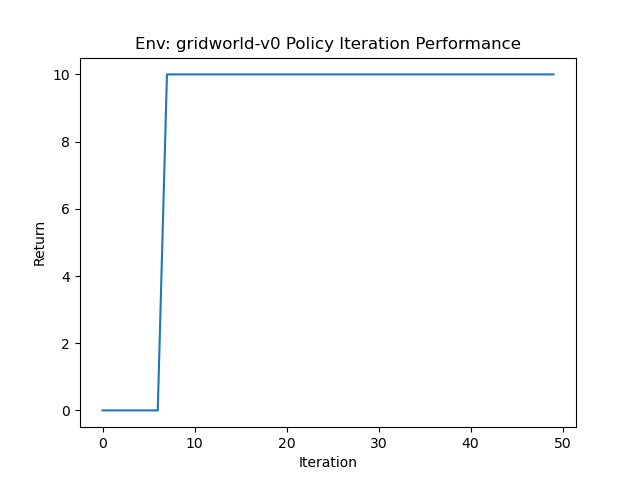
\includegraphics[width=\textwidth]{../figures/gridworld-v0_deterministic_pi.png}
        \caption{Improvement over time of policy values on the \texttt{GridWorld(0)} environment.}
\end{figure}



\end{enumerate}


%--------------------------------------------------------------------------------
%--------------------------------------------------------------------------------
%--------------------------------------------------------------------------------
\newpage 
\noindent {\bf 3. Discretization}
%--------------------------------------------------------------------------------
%--------------------------------------------------------------------------------
%--------------------------------------------------------------------------------

\begin{enumerate}[(a)]

\item {\bf [20pts] Nearest-neighbor interpolation.} Value Iteration can only work when the state and action spaces are discrete and finite. If these assumptions do not hold, we can approximate the problem domain by coming up with a discretization such that the previous algorithm is still valid. The \textt{MountainCar} domain, as described in class, has a continuous state space that will prevent us from using value or policy iteration to solve it directly. One of the solutions that we came up with for this was \emph{nearest-neighbor interpolation}, where we discretize the actual state space $S$ into finitely many states $\Xi={\xi_1, \xi_2,...,\xi_n}$, and act as if we are in the $\xi$ nearest to our actual state $s$.

Implement Value Iteration with nearest-neighbor interpolation on the \textt{MountainCar} domain. You will need to add code in \texttt{code/continuous\_solution.py} below the lines \texttt{if self.\_mode == `nn'}. Run the script and report the state value heatmap for \texttt{MountainCar}, discretizing each dimension of the state space (position and velocity) into 21, 51, and 151 bins.

\begin{figure}[h!]
    \centering
    \begin{subfigure}{0.3\textwidth}
        \centering
        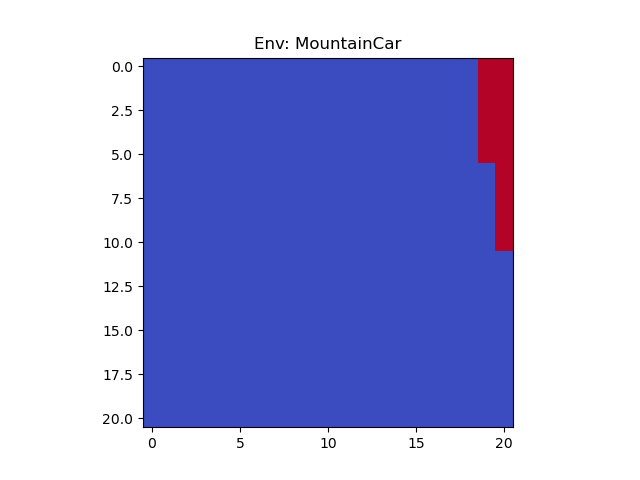
\includegraphics[width=\textwidth]{../figures/MountainCar_nn_21.png}
        \caption{Heatmap of state values after 150 iterations of the value iteration algorithm on the \texttt{MountainCar} environment using nearest-neighbor interpolation. The continuous state space has been discretized into 21x21 states.}
    \end{subfigure}
    \hspace{0.1 in}
    \begin{subfigure}{0.3\textwidth}
        \centering
        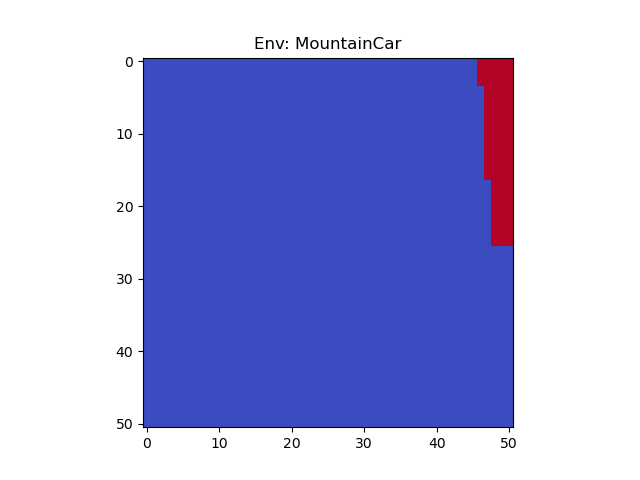
\includegraphics[width=\textwidth]{../figures/MountainCar_nn_51.png}
\caption{Heatmap of state values after 150 iterations of the value iteration algorithm on the \texttt{MountainCar} environment using nearest-neighbor interpolation. The continuous state space has been discretized into 51x51 states.}
    \end{subfigure}
        \hspace{0.1 in}
    \begin{subfigure}{0.3\textwidth}
        \centering
        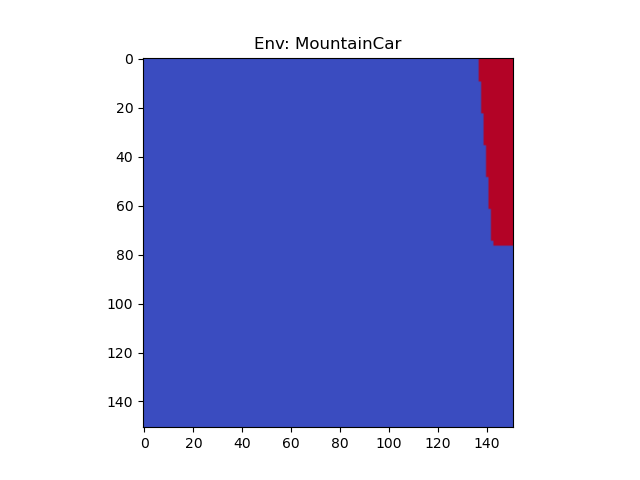
\includegraphics[width=\textwidth]{../figures/MountainCar_nn_151.png}
\caption{Heatmap of state values after 150 iterations of the value iteration algorithm on the \texttt{MountainCar} environment using nearest-neighbor interpolation. The continuous state space has been discretized into 151x151 states.}
\end{subfigure}
\end{figure}

\newpage
\item {\bf [10pts] n-linear interpolation.} Nearest-neighbor interpolation is able to approach the optimal solution if you use a fine-grained approximation, but doesn't scale well as the dimensionality of your problem increases. A more powerful discretization scheme that we discussed in class is \emph{n-linear interpolation}, an $n$-dimensional analogue of linear interpolation. Add your code within \texttt{code/continuous\_solution.py} below the line \texttt{if self.\_mode == `linear'}. Just as before, report the state value heatmap for \texttt{MountainCar} with discretization resolutions of 21, 51, and 151 points per dimension.

\begin{figure}[h!]
    \centering
    \begin{subfigure}{0.3\textwidth}
        \centering
        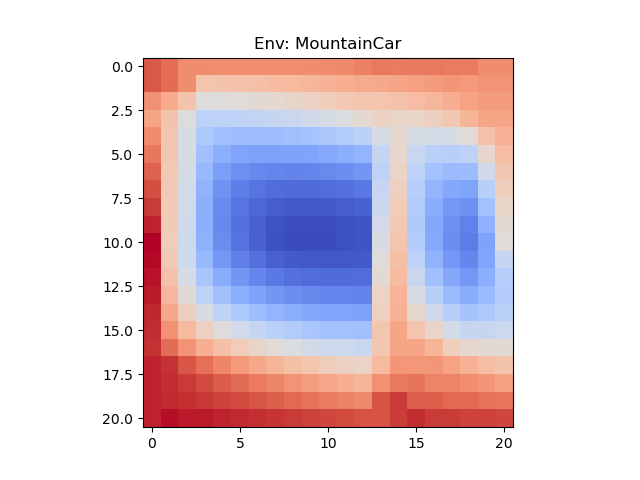
\includegraphics[width=\textwidth]{../figures/MountainCar_linear_21.png}
        \caption{Heatmap of state values after 150 iterations of the value iteration algorithm on the \texttt{MountainCar} environment using n-linear interpolation. The continuous state space has been discretized into 21x21 states.}
    \end{subfigure}
    \hspace{0.1 in}
    \begin{subfigure}{0.3\textwidth}
        \centering
        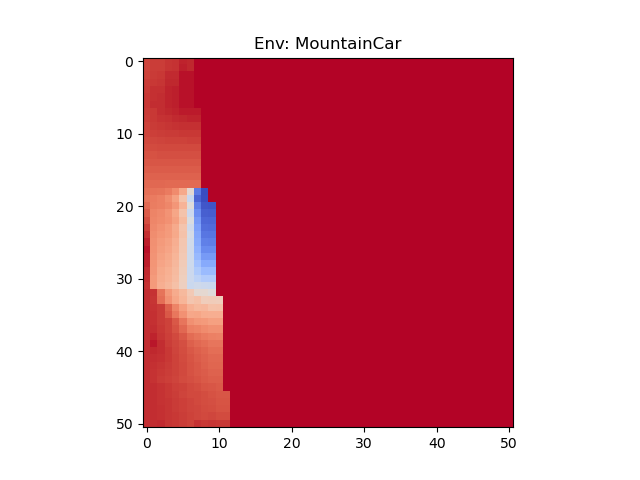
\includegraphics[width=\textwidth]{../figures/MountainCar_linear_51.png}
\caption{Heatmap of state values after 150 iterations of the value iteration algorithm on the \texttt{MountainCar} environment using n-linear interpolation. The continuous state space has been discretized into 51x51 states.}
    \end{subfigure}
        \hspace{0.1 in}
    \begin{subfigure}{0.3\textwidth}
        \centering
        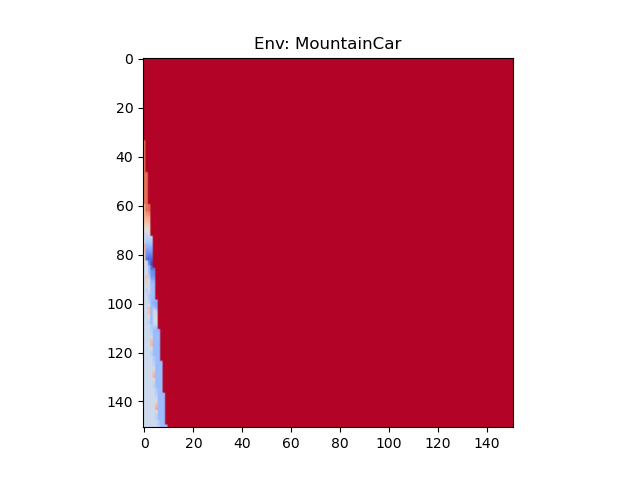
\includegraphics[width=\textwidth]{../figures/MountainCar_linear_151.png}
\caption{Heatmap of state values after 150 iterations of the value iteration algorithm on the \texttt{MountainCar} environment using n-linear interpolation. The continuous state space has been discretized into 151x151 states.}
\end{subfigure}
\end{figure}



\item {\bf [10pts] Look-ahead policies \textbf{(GRAD)}.} Using Value Iteration, we can find the expected reward when acting optimally for every state in our problem domain... but it is fairly common that we won't need to solve for all of these values in practice. In these cases, we only really need to be able to compute a policy for a subset of the overall state space, suggesting that we won't really need to run Value Iteration until it's fully converged or over a fine-grained state space approximation.

An alternative to this is to purposefully choose a smaller number of discretized states or to run it for fewer iterations than necessary for convergence, but increase our algorithm's power by leveraging look-ahead. When using look-ahead, we optimize over taking a sequence of $k$ actions instead of just one, using the sum of near-term reward plus the value achieved from the state we expect to end up in after $k$ steps. For continuous domains, this value will be approximated by the discretization of the state we expect to end up in. After solving this optimization problem (for $k$ actions), we only take the first action and repeat the process. Add your code to \texttt{code/continuous\_solution.py} below the line \texttt{        if self.\_lookahead\_steps > 0}.

Plot the learning curves for policies with look-ahead horizon values of 1, 2, and 3 for the \texttt{MountainCar} environment with a discretization of 51x51. The vertical axis should be actual reward received over a run of the domain, while the horizontal axis should indicate which training iteration it was performed with.

\end{enumerate}

\begin{figure}[h!]
    \centering
        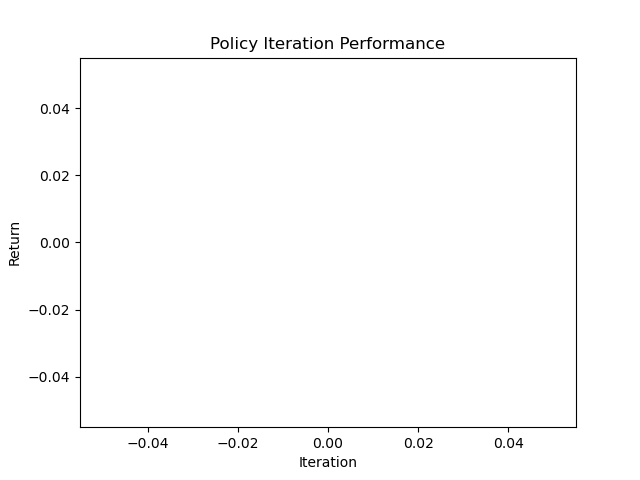
\includegraphics[width=\textwidth]{../figures/lookahead_mc.png}
        \caption{Policy performance over training iteration for different look-ahead horizons in the \texttt{MountainCar} environment.}
\end{figure}

\end{document}
